\documentclass[crop,tikz]{standalone}
\usepackage{tkz-euclide}
\usetikzlibrary{arrows.meta}
\usetkzobj{all}
\usetikzlibrary{shapes}


\tikzstyle{myarrows}=[line width=1mm,draw=blue,-triangle 45,postaction={draw, line width=3mm, shorten >=4mm, -}]
\begin{document}

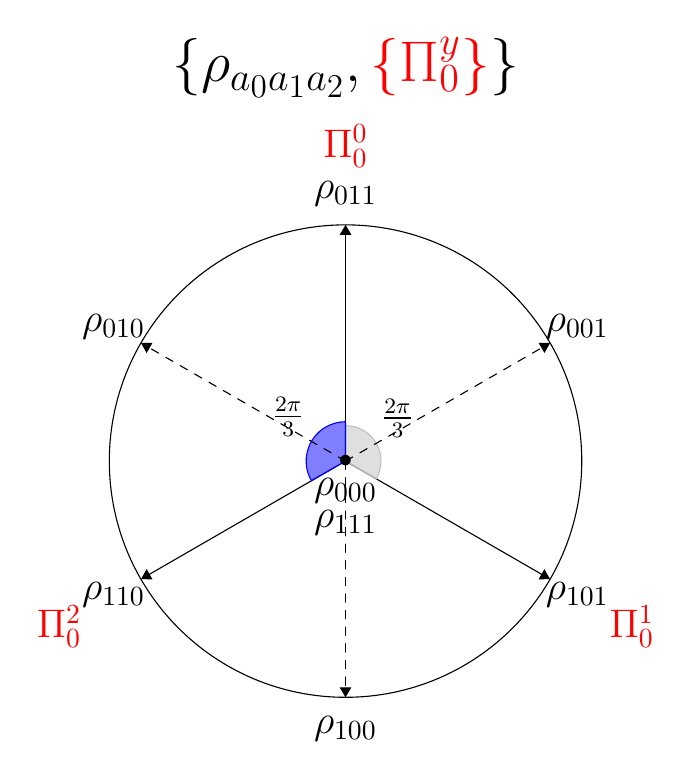
\begin{tikzpicture}[line cap=round, line join=round, >=Triangle]

\begin{scope}[ shift={(0,0)}]
\draw  (0,0) ellipse (3 and 3);


\draw[->]  (0,0) -- (0,3);
\draw (0,3.4) node {\Large $\rho_{011}$};
\draw (0,4) node {\Large \color{red} $\Pi^0_0$};




\begin{scope}[rotate=-120]    
	\draw[->]  (0,0)  -- (0,3);
	\draw (0,3.4) node {\Large $\rho_{101}$};
	\draw [lightgray, fill, fill opacity=0.5]  (0,0) -- (90:0.45) arc (90:210:0.45) -- cycle;
	\node at (-0.8,0.3) {\large $\frac{2\pi}{3}$};
	\draw (0,4.2) node {\Large \color{red} $\Pi^1_0$};

\end{scope}



\begin{scope}[rotate=120]    
	\draw[->]  (0,0)  -- (0,3);
	\draw (0,3.4) node {\Large $\rho_{110}$};
	\draw [shift={(0,0)}, blue, fill, fill opacity=0.5] (0,0) -- (90:0.5) arc (90:-30:0.5) -- cycle;
\node at (0.85,0.35) {\large $\frac{2\pi}{3}$};
	\draw (0,4.2) node {\color{red}  \Large $\Pi_0^2$};
\end{scope}


\begin{scope}[rotate=60]    
	\draw[->,dashed]  (0,0)  -- (0,3);
	\draw (0,3.4) node {\Large $\rho_{010}$};
\end{scope}

\begin{scope}[rotate=-60]    
	\draw[->,dashed]  (0,0)  -- (0,3);
	\draw (0,3.4) node {\Large $\rho_{001}$};
\end{scope}
\begin{scope}[rotate=180]    
	\draw[->,dashed]  (0,0)  -- (0,3);
	\draw (0,3.4) node {\Large $\rho_{100}$};
\end{scope}

\node at (0,5) {\huge $\{\rho_{a_0a_1a_2},{\color{red} \{\Pi^y_0\}}\}$ };
\node[] at (0,0) { $\bullet$};
\node[below] at (0,-0.1) {\Large $\rho_{000}$};
\node[below] at (0,-0.5) {\Large $\rho_{111}$};
\end{scope}

%---------------------------------------------------------------------------------------------------
%\begin{scope}[ shift={(8,0)}]
%\draw  (0,0) ellipse (3 and 3);


%\draw[->]  (0,0) -- (0,3);
%\draw (0,3.4) node {\Large $\Pi^0_0$};




%\begin{scope}[rotate=-120]    
%	\draw[->]  (0,0)  -- (0,3);
%	\draw (0,3.4) node {\Large $\Pi^1_0$};
%	\draw [lightgray, fill, fill opacity=0.5]  (0,0) -- (90:0.45) arc (90:210:0.45) -- cycle;
%	\node at (-0.8,0.3) {\large $\frac{2\pi}{3}$};
%\end{scope}




%\begin{scope}[rotate=120]    
%	\draw[->]  (0,0)  -- (0,3);
%	\draw (0,3.4) node {\Large $\Pi^2_0$};
%	\draw [shift={(0,0)}, fill] (0,0) -- (90:0.5) arc (90:-30:0.5) -- cycle;
%\node at (0.85,0.35) {\large $\frac{2\pi}{3}$};
%\end{scope}



%\node at (0,4.5) {\huge $\{\Pi^y_k\}$ };
%\end{scope}

%---------------------------------------------------------------------------------------------------


\end{tikzpicture}

\end{document}